%\documentclass[11pts,letter]{book}
\documentclass[letter,12pt,times,numbered,print,index]{Classes/PhDThesisPSnPDF}

\usepackage[utf8]{inputenc}
\usepackage[spanish]{babel}
\usepackage[pdftex]{graphicx}
\usepackage{listings}
\usepackage{verbatim} 
\usepackage{color}
\usepackage{enumerate}
%\usepackage{cite}
\usepackage[table,xcdraw]{xcolor}
%paquete para el cronograma en gantt
\usepackage{pgfgantt}
%Paquetes para rotar imagenes.
\usepackage{rotating}
\usepackage{pdflscape}
\usepackage{array}
\usepackage{bera}% optional: just to have a nice mono-spaced font
\usepackage{listings}
\usepackage{xcolor}
\usepackage{tabu}




\colorlet{punct}{red!60!black}
\definecolor{background}{HTML}{EEEEEE}
\definecolor{delim}{RGB}{20,105,176}
\colorlet{numb}{magenta!60!black}


\lstdefinelanguage{json}{
    basicstyle=\normalfont\ttfamily,
    numbers=left,
    numberstyle=\scriptsize,
    stepnumber=1,
    numbersep=8pt,
    showstringspaces=false,
    breaklines=true,
    frame=lines,
    backgroundcolor=\color{background},
    literate=
     *{0}{{{\color{numb}0}}}{1}
      {1}{{{\color{numb}1}}}{1}
      {2}{{{\color{numb}2}}}{1}
      {3}{{{\color{numb}3}}}{1}
      {4}{{{\color{numb}4}}}{1}
      {5}{{{\color{numb}5}}}{1}
      {6}{{{\color{numb}6}}}{1}
      {7}{{{\color{numb}7}}}{1}
      {8}{{{\color{numb}8}}}{1}
      {9}{{{\color{numb}9}}}{1}
      {:}{{{\color{punct}{:}}}}{1}
      {,}{{{\color{punct}{,}}}}{1}
      {\{}{{{\color{delim}{\{}}}}{1}
      {\}}{{{\color{delim}{\}}}}}{1}
      {[}{{{\color{delim}{[}}}}{1}
      {]}{{{\color{delim}{]}}}}{1},
}

% ************************ Thesis Information & Meta-data **********************
%% The title of the thesis
\title{PROTOTIPO PARA LA ADMINISTRACIÓN CENTRALIZADA DE DATAPOWER}

%\texorpdfstring is used for PDF metadata. Usage:
%\texorpdfstring{LaTeX_Version}{PDF Version (non-latex)} eg.,
%\texorpdfstring{$sigma$}{sigma}

%% Subtitle (Optional)
\subtitle{}

%% The full name of the author
\author{OSCAR DARIO PABÓN RODRIGUEZ \\ Código: 20161099034 \\ JAVIER ALEJANDRO HERNÁNDEZ SANTANA \\ Código: 20161099029}

%% Department (eg. Department of Engineering, Maths, Physics)
%\dept{Department of Engineering}

%% University and Crest
\university{Universidad Distrital Francisco José de Caldas}
\crest{
\includegraphics[width=0.25\textwidth]{Imagenes/LogoUdistrital.png}}

%% You can redefine the submission text:
% Default as per the University guidelines:
% ``This dissertation is submitted for the degree of''
\renewcommand{\submissiontext}{Trabajo para optar por el titulo de:}

%% Full title of the Degree
\degree{Ingeniero de Software}

%% College affiliation (optional)
%\college{King's College}

%% Submission date
% Default is set as {\monthname[\the\month]\space\the\year}
%\degreedate{September 2014} 

%% Meta information
\subject{LaTeX} \keywords{{LaTeX} {Tesis Ingenieria de software datapower prototipo administracion centralizada} {ingenieria de software} {Universidad Distrital Francisco José de Caldas}}


\begin{document}
	\maketitle
	%\begin{titlepage}
	
	\begin{center}
		\textbf{Prototipo para la administración centralizada de Datapower}\\
		\vspace*{0.5in}
		\vspace*{1in}
		\begin{figure}[htb]
			\begin{center}
				
\includegraphics[width=5cm]{./Imagenes/LogoUdistrital.png}
			\end{center}
		\end{figure}
		
		%%%%%%%
		\textbf{Oscar Dario Pabon Rodriguez\\
				Código: 20161099034 \\
				Javier Alejandro Hernandez Santana\\
				Código: 20161099029 \\
				\vspace{2in}
				Universidad Distrital Francisco José de Caldas\\
				Facultad de Ingeniería\\
				Especialización En Ingeniería De Software\\
				Bogotá D.C. 2016	
				}
	\end{center}
\end{titlepage}
	\tableofcontents
	\listoffigures
	\listoftables
	%divison de la estructura
	%\part*{Introducción}
	\mainmatter
	\chapter{Introducción}
\section*{Introducción}
En la actualidad, un administrador de infraestructura de una organización debe garantizar que las plataformas estén en funcionamiento 7x24, debido a la gran cantidad de transacciones que pasan sobre las diversas máquinas de la infraestructura.
\newline
El Datapower ®, como plataforma de integración, al ser un punto central en la infraestructura de la arquitectura SOA, su administrador debe garantizar que su configuración sea la adecuada y se encuentre sincronizada en todo el ambiente, que tengan los protocolos de seguridad adecuados y el enrutamiento de los servicios web correcto para cada transacción.
\newline
En el momento en que los volúmenes de transacciones aumenta y se necesita realizar acciones sobre las plataformas, es ahí donde se puede perder el control y caer en errores involuntarios, ya sea por la presión de los superiores, el afán de actuar en pro de dar soluciones ágiles o simplemente por las tareas repetitivas que se llevan a cabo cuando se procese a interactuar con cada uno de los Datapower ®.
Con el fin de evitar estos problemas, se plantea una solución que consiste en una aplicación web, la cual centraliza las tareas sobre las plataformas de IBM con el fin de unificar en un solo punto las tareas de los administradores.
	%\part{Contextualizacion de la investigacion}
	
\chapter{Descripción de la investigación}
\newpage
\section{Título y definición del tema de investigación}
\subsection*{Título}
Prototipo para la administración centralizada de Datapower.
\section{Estudio del problema de investigación}
\subsection{Planteamiento del problema}
Datapower , al ser un tipo de plataforma de alta disponibilidad debe ser confiables en su configuración debido a que muchas de las transacciones pasan por estos,  debe contar con las parametrizaciones exactas para garantizar que las transacciones fluyan hacia al destino configurado de manera correcta y no genere rechazos o enrutamientos errados. Existe un margen de riesgo alto en la configuración de cada equipo debido a que se debe hacer uno a uno manualmente, por parte de los administradores de la plataforma, como tal, no existe un punto centralizado que dé la confiabilidad de hacer la misma parametrización para todos los Datapower  de manera centralizada. 
\newline
Contando con una herramienta que facilite estos trabajos repetitivos, se disminuye drásticamente los tiempos de parametrización de toda la plataforma. Adicional a esto, podemos contar con un monitoreo en tiempo real que permita observar el comportamiento de cada equipo, en caso de requerirlo. Como valor agregado, se contarán con métricas que apoyen a la toma de decisiones y el gobierno de los servicios.
\subsection{Formulación del problema}
¿Cómo a través de una herramienta puedo administrar y monitorear a los diferentes Datapower  desde un punto centralizado?
\subsection{Sistematización del problema}
\begin{itemize}
    \item ¿Cuáles son las principales acciones que se deberían identificar para la administración que se podrían automatizar para cada uno de los Datapower?
    \item ¿Cuál es la mejor forma de almacenar los datos generados por las plataformas para mostrar información en tiempos oportunos?
    \item ¿Cómo se puede realizar un piloto teniendo en cuenta la limitante de no tener un Datapower  físico?
\end{itemize}
\newpage
\section{Objetivos de la investigación}
\subsection{Objetivo general.}
Construir un prototipo que permita desde un solo punto gestionar la administración y monitoreo de cada uno de los Datapower por medio de las interfaces de administración que estos ofrece
\subsection{Objetivos específicos.}
\begin{itemize}
    \item Identificar las principales operaciones qué se requieran, mediante entrevistas a los diferentes administradores de la plataforma, para tener un punto base de cuáles operaciones se van a centralizar.
    \item Diseñar un modelo de información de los diferentes atributos del sistema, analizando los parámetros y registros qué proporciona la plataforma para generar las métricas del sistema y su comportamiento.
    \item Realizar un piloto al prototipo, con 4 máquinas virtuales simultáneas de los Datapower  que asemeje un entorno real y así poder comprobar su funcionalidad.
\end{itemize}
\newpage
\section{Justificación de la investigación}
\subsection{Justificación práctica}
Los sistemas Datapower  pueden ser utilizadas en diferentes organizaciones y proveen seguridad y enrutamiento en las transacciones, generalmente se encuentran en alta disponibilidad y son gemelos en configuración y parámetros, en donde para su administración es necesario ingresar a cada uno por medio de una terminal a realizar las operaciones necesarias para su administración, esta tarea se puede volver algo dispendioso y es a su vez riesgoso, ya qué se puede incurrir en error humano y configurarlos de diferente manera. En la actualidad existen diferentes alternativas para centralizar la configuración de estos sistemas, pero estas alternativas no cubren las necesidades de un administrador en su día a día, de ahí la necesidad de crear una aplicación web que permita, tanto administrar como monitorear cada uno de las estaciones de una forma más eficiente y así facilitar la labor del administrador en la parametrización de cada Datapower  por cada ambiente de la organización.
\newpage
\section{Hipótesis de trabajo}
Una aplicación web que permita realizar todos los procesos administrativos que se ejecutan a los Datapower  de forma centralizada, podría solucionar los siguientes inconvenientes encontrados en el proceso de levantamiento de información:
\begin{itemize}
    \item Es necesario repetir la misma configuración en las diversas máquinas, produciendo re trabajo innecesario.
    \item Se incurre en el riesgo de realizar mal la configuración manual de algún componente en alguna de las máquinas, causando posibilidad de errores en la configuración.
    \item Cada máquina genera sus propios logs y trazas dificultando analizar la información para toma de decisiones.
    \item Por malas configuraciones, se producen fallos de conectividad, produciendo fallos críticos en las operaciones.
    \item Cuando se decide aumentar las plataformas, aumenta la cantidad de tareas repetitivas de cada una, aumentando el tiempo en vincular nuevos dispositivos.
\end{itemize}
\newpage

	\section{Marco de referencia}
\subsection{Marco teórico}
IBM Datapower Es una plataforma de integración y seguridad comercializada por IBM, diseñada específicamente para cargas de trabajo móviles, cloud, API (interfaz de programación de aplicaciones), web, SOA (arquitectura orientada a servicios) y B2B (business-to-business).
\\
Actualmente en el mercado existen varias alternativas a Datapower ®, que cumplen con las mismas capacidades de integración de web services 
\begin{itemize}
    \item WSO2 Carbón, distribuido por WS02 
    \item Cisco ACE XML Gateway, distribuido por Cisco
    \item CA API Gateway
    \item Axway API Gateway, distribuido por Axway.
\end{itemize}


\begin{table}[h]
\caption{Comparativo Características plataformas similares a Datapower}
\begin{tabular}{llllll}
\hline
Plataforma & \begin{tabular}[c]{@{}l@{}}Procesamiento\\ XML\end{tabular} & \begin{tabular}[c]{@{}l@{}}Transformación\\ entre\\ protocolos\end{tabular} & \begin{tabular}[c]{@{}l@{}}Manejo\\ Certificados\end{tabular} & \begin{tabular}[c]{@{}l@{}}Manejo\\ REST\end{tabular} & WS-Security \\ 
\hline
Datapower        & SI                                                          & SI                                                                          & SI                                                            & NO                                                    & SI          \\
WSO2       & SI                                                          & SI                                                                          & NO                                                            & SI                                                    & NO          \\
Cisco      & SI                                                          & SI                                                                          & SI                                                            & NO                                                    & NO          \\
CA         & SI                                                          & SI                                                                          & SI                                                            & NO                                                    & SI          \\
Axway      & SI                                                          & SI                                                                          & SI                                                            & SI                                                    & SI         
\end{tabular}
\end{table}



\subsubsection{IBM Datapower ® SOMA SOAP Configuration Management}
SOMA es una interfaz de configuración que provee Datapower \cite{id1} para labores de automatización de configuración de elementos. Presenta mediante SOAP todas las operaciones que se pueden llegar a realizar en un Datapower ®, esta interfaz no se encuentra completamente documentada por parte de IBM, se limita a presentar únicamente ejemplos prácticos de cómo utilizar algunas operaciones de las más de 100 expuestas en el contrato del servicio SOMA.
\subsubsection{IBM Datapower ® Gateway script}
Es un modelo de programación definido para Datapower ® en firmware 7.2 y superiores, basado en ECMACScript que permite mediante lenguaje 
JavaScript desarrollar funcionalidades y reglas de procesamiento sobre Datapower ®, sin dejar de lado la capacidad de procesamiento XML, ya que los script son interpretados a lenguaje XSLT para aprovechar el procesamiento de XML por hardware de Datapower ®.
\subsubsection{Arquitectura orientada a servicios SOA}
La definición de arquitectura, según la ISO42010, dice que son conceptos fundamentales y propiedades de un sistema, en su ambiente, concretados en sus elementos, relaciones y principios, que guían su diseño y evolución. Para la arquitectura SOA (Servicie Oriented Architecture), estos elementos son los servicios que enmascaran las funcionalidades que ofrece. 
\newline
Este tipo de arquitecturas define unos elementos clave para su funcionalidad:
\begin{itemize}
    \item Servicio
    \item Composición
    \item Contrato
    \item Interfaz
    \item Declaración
    \item Modos de operación
    \item Interoperabilidad
\end{itemize}
\subsection{Marco Conceptual}
El proyecto se basa principalmente en metodologías de desarrollo web, debido a que lo que se quiere es centralizar en un solo punto, para que el administrador de las plataformas de Datapower ®, donde quiera que esté, que pueda administrar, monitorear y generar las métricas deseadas.
\subsubsection{Aplicaciones web}
Son sistemas de información que dan ciertas ventajas sobre las aplicaciones Stand-alone o aplicaciones de escritorio, como lo es manejo distribuido, sencillez en la instalación y presentaciones más llamativas para el usuario final. La principal herramienta de estos sistemas de información son los navegadores y en la actualidad cada navegador tiene su propio motor de Java Script y soporte para HTML5.
\subsubsection{Frameworks de desarrollo Web}
Existen varios frameworks para el desarrollo de estas aplicaciones, los cuales facilita la construcción de plataformas web, dependiendo de la experiencia del desarrollador. Existen unos que son muy especializados a lenguajes de alto nivel, como los son GWT y JSF (Java Server Faces \cite{id3}), por mencionar algunos.
\newline
GWT
\newline
GWT es un framework de Google, el cual realiza una transformación de código Java a código java script, para aqu
ellos que desean desarrollar aplicaciones web, teniendo un vago conocimiento en HTML, java script y CSS
\newline
JSF (Java Server Faces)
\newline
JSF es un framework creado para desarrollar aplicaciones Java basadas en el patrón MVC, tiene 2 funciones principales, una es la de generar una interfaz de usuario en HTML, esta interfaz en el servidor es representada a través de un árbol de componentes, existe una relación 1 a 1 entre el árbol de componentes y la interfaz de usuario. La segunda función es responder a eventos generados por el usuario.
\newline
Por otro lado tenemos frameworks que son dedicados 100 por ciento al lado del navegador, que igualmente facilitan la labor del desarrollador, por mencionar algunos tenemos Angular, JQeury, Polymer, React, Backbone, Ember, entre otros.
\subsubsection{XML}
Es un metalenguaje diseñado para la organización y etiquetado de documentos, creado por el W3C (Word Wide Web Consortium). Entre sus principales ventajas:
\begin{itemize}
    \item Fácil procesamiento
    \item Separa radicalmente el contenido y el formato de presentación
    \item Diseñado para cualquier lenguaje
\end{itemize}
\subsubsection{JavaScript}
Es un lenguaje de programación orientado a objetos multiplataforma, liviano y pequeño. Posee librerías estándar de objetos, como lo son Array, Date, y Math, al igual que un conjunto central de elementos del lenguaje, tales como operadores, estructuras de control y sentencias.
\subsubsection{Estado del Arte.}
En la actualidad existen 3 herramientas que facilitan la administración de la plataforma.
\newline
Datapower ® Buddy 
\newline
“DPBuddy es una herramienta de pago para automatizar la administración y el manejo de IBM Datapower ®. Automatiza la construcción, el despliegue y la entrega de configuraciones y archivos relacionados“ 
\newline
Urban Code
\newline
“IBM Urban Code Deploy instrumenta y automatiza el despliegue de aplicaciones, configuraciones de middleware y cambios en bases de datos en entornos de desarrollo, pruebas y producción. Este software permite que su equipo lleve a cabo despliegues on demand, tan a menudo como sea necesario o conforme a una planificación y con autoservicio. UrbanCode Deploy puede ayudar a su equipo a acelerar el tiempo de lanzamiento al mercado, reducir los costes y los riesgos” %\cite{ol5}
\newline
WebSphere Appliance Management Center for WebSphere Appliances (WAMC)
\newline
Provee la capacidad de administrar diversos appliance de manera centralizada, realizando las actividades principales requeridas por los Datapower ®, a nivel de administración, como:
\begin{itemize}
    \item Cargue de backups
    \item Instalación de firmwares.
    \item Monitoreo del appliance
    \item Soporte de diversas versiones de Datapower ®.
\end{itemize}
Actualmente WAMC está fuera de soporte y descontinuado.
Comparativo de las 3 alternativas existentes, contra las prestaciones que tendrá el prototipo a construir:
\newline

\begin{sidewaystable}
	\begin{table}[h]
		\caption{Comparativo de las 3 herramientas alternativas existentes.}
		\begin{tabular}{llllll}
			\hline
			\multicolumn{1}{c}{Plataforma} & \multicolumn{1}{c}{\begin{tabular}[c]{@{}c@{}}Administración\\ Centralizada\end{tabular}} & \multicolumn{1}{c}{GUI Usuario} & \multicolumn{1}{c}{\begin{tabular}[c]{@{}c@{}}Scripts\\ automatización\end{tabular}} & \multicolumn{1}{c}{Monitoreo} & \multicolumn{1}{c}{\begin{tabular}[c]{@{}c@{}}Manejo Logs de\\ la plataforma\end{tabular}}  \\
			\hline
			DPBuddy                        & SI                                                                                        & NO                              & SI                                                                                   & NO                            & NO                                                                                         \\
			Urban Code                     & NO                                                                                        & SI                              & SI                                                                                   & NO                            & NO                                                                                         \\
			WAMC                           & SI                                                                                        & SI                              & NO                                                                                   & SI                            & NO                                                                                         \\
			Prototipo                      & SI                                                                                        & SI                              & SI                                                                                   & NO                            & SI                                                                                        
		\end{tabular}
	\end{table}
\end{sidewaystable}

\newpage
	\section{Aspectos metodologicos}
\subsection{Tipo de estudio}
El tipo de estudio identificado para el proyecto es el Descriptivo, debido a que el problema se centra en mejorar un proceso existente de administración de plataformas, el cual es repetitivo, y se desea obtener la manera de centralizar los procesos.
\subsection{Método de investigación}
	Para poder llegar al conocimiento deseado sobre el problema, se trabajara con dos metodologías tradicionales, estas son:
\begin{itemize}
    \item Método de observación.
    \item Método de Análisis.
\end{itemize}
La observación como medio para determinar las principales características  que abarca el problema en su medio ambiente, tomando las experiencias de los interesados y así tener una base de conocimiento que facilite contextualizar el problema.
\newline
El método analítico nos permite determinar diferentes variables, identificando cada parte del problema en cuestión,  permitiéndonos llegar a una explicación completa del problema y con base en la causa-efecto obtenida plantear la solución al problema.
\subsection{Fuentes y técnicas para la recolección de la información}
	Con el objetivo de recolectar información determinante en pro del desarrollo del proyecto, se establecen entrevistas con los interesados principales, con el fin de obtener detalles en el proceso. Otra herramienta clave es la observación, el cual brinda identificar las características del problema en el medio ambiente que lo rodea.
\newpage
\subsection{Cronograma}
%%\subsection{Tareas}
%%\begin{figure}[th!]
%%        \centering
%%        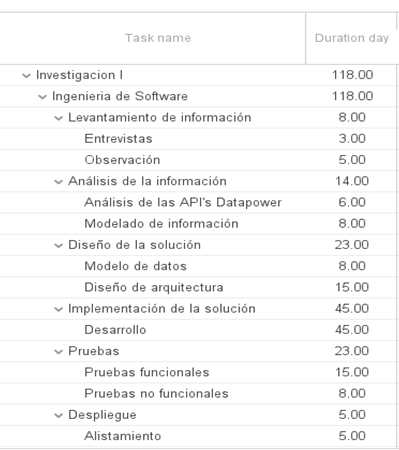
\includegraphics[width=1.0\textwidth]{parte1/img/tareas.png}
%%        \caption{Tareas}
%%    \end{figure}
\subsection*{Diagrama de grantt}

\begin{figure}[th!]
    \begin{ganttchart}[
            vgrid, 
            hgrid,
            y unit chart = .5cm,
            x unit = .6cm
            ]{1}{17}
        \ganttset{bar height=.2}{group height=.4}{group label node/.append style={align=rigth}}
        \gantttitle{Prototipo Administración centralizada DP.}{17} \\
        \gantttitle{SEMANAS}{17} \\
        \gantttitlelist{1,...,17}{1}\\
        \ganttgroup{Levantamiento Información}{1}{2} \\
            \ganttbar{Entrevistas}{1}{1} \\
            \ganttlinkedbar{Observación}{2}{2} \\
        \ganttgroup{Análisis de Información}{2}{3} \\
            \ganttbar{Análisis de las API de DP}{2}{2} \\
            \ganttlinkedbar{Modelado de la información}{3}{3} \\
        \ganttgroup{Diseño de la solución}{4}{7} \\
            \ganttbar{Modelado de datos}{4}{5} \\
            \ganttlinkedbar{Diseño de la arquitectura}{6}{7} \\
        \ganttgroup{Implementación de la solución}{7}{13} \\
            \ganttbar{Desarrollo Fase 1}{7}{11} \\
            \ganttlinkedmilestone{Primero prototipo}{11} \\
            \ganttlinkedbar{Desarrollo Fase 2}{12}{13} \\
        \ganttgroup{Pruebas}{14}{16} \\
            \ganttbar{Pruebas Funcionales}{14}{15} \\
            \ganttlinkedmilestone{Segundo prototipo}{15} \\
            \ganttlinkedbar{Pruebas No Funcionales}{16}{16} \\
        \ganttgroup{Despliegue}{17}{17} \\
            \ganttbar{Alistamiento}{17}{17} \\
    \end{ganttchart}
    \caption{Diagrama de grantt}
\end{figure}
	\section{Alcances, limitaciones y resultado esperado}
\subsection{Alcances}
El alcance de la investigación se centrará únicamente para el producto Datapower de IBM para la edición virtual de estudio, se enfocará en las operaciones de administración y monitoreo resultantes de las observaciones y entrevistas realizados a diferentes administradores de la herramienta.
\newline
\subsection{Limitaciones}
\begin{itemize}
  \item Dado que no se usar una plataforma física, se cuenta únicamente con una versión virtual de IBM Datapower
  \item La documentación de las Apis del Datapower no es muy extensa.
  \item No se comprarán licencias para el desarrollo del prototipo
\end{itemize}   
\subsection{Resultados esperados}
\begin{itemize}
  \item Establecer una lista de actividades comunes que realizan los administradores de Datapower
  \item Establecer los atributos de monitoreo que los administradores de Datapower utilizan en su día a día para garantizar el correcto funcionamiento del appliance.
  \item Contar con el prototipo de una herramienta web que permita realizar la administración de acuerdo a los resultados de los sondeos realizados y que presente el monitoreó que más conciernan a los administradores entrevistados.  
\end{itemize}
\newpage
	
	
	%\part{Desarrollo De La Investigacion}
	\chapter{Desarrollo de la investigacion}

\section{Desarrollo de la investigacion}
Para el desarrollo de este proyecto se utilizaron cuestionarios o entrevistas por escrito con un total de 24 interrogantes en donde se buscaba profundizar en la interacción del usuario del Datapower y las operaciones que suelen realizar comúnmente.
Toda la información recolectada se analizará con el fin de detectar las principales actividades que realiza el administrador de plataformas Datapower ®, y así poder lograr obtener un común denominador de las tareas más importantes de cada administrador entrevistado.
\newline
El tratamiento consiste en tomar todas las tareas y las variables que desean monitorear recolectadas de las entrevistas que se van a realizar a los administradores de las plataformas, junto con una valoración de importancia de cada una. A partir de esta información, se obtendrá el común denominador y se organizara de la más a la menos relevante. Con esta lista ordenada, se tomaran los 10 principales resultados de cada lista para el desarrollo del prototipo.
\subsection{Recolección y análisis de la información}
Se consiguió un grupo de personas que trabajan con la plataforma Datapower en diferentes empresas para obtener diversos puntos de vista de las tareas qué realizan en los Datapower de sus compañías. 
\newline
Se realizaron 24 preguntas para determinar las operaciones comunes qué realizan los administradores, de las cuales se detectaron tareas principales que cada administrador debe realizar y no están sistematizadas en la actualidad.
\subsubsection{Perfil de los entrevistados}
Las personas entrevistadas son bien administradores o desarrolladores sobre el Datapower, interactúan en su día a día con la plataforma, un grupo de 6 personas entrevistadas:
\\
\\
\begin{tabu}{ X[l]  X[l] }
Liliana Ortegón: &  Administradora Datapower Banco De Bogotá \\
Diego Arias: &  Desarrollador y administrador Datapower Banco De Bogotá \\
Manuel Jiménez: &  Desarrollador Datapower Banco De Bogotá \\
German Aya: &  Administrador Datapower Banco Av. villas \\
Javier Hernández: &  Administrador Datapower Banco Av. villas. \\
Alexander Forero Lozano: &  Administrador Datapower ATH.    
\end{tabu}


\subsubsection{Análisis de los resultados obtenidos}
Al realizar entrevistas con preguntas abiertas, no es posible realiza la tabulación de la información, sin embargo se realiza una consolidación en donde se identifica la información concerniente a la investigación y los puntos relevantes para el desarrollo del producto, adicional se logra evidenciar la necesidad de una herramienta que permita manejar/ administrar maquinas Datapower desde un punto central.
\newline
A continuación se detallan los puntos mas relevantes obtenidos de las 6 entrevistas realizadas.
\begin{description}
\item [Máquinas Datapower qué manejan] 1 - 4
\item [Dominios qué puede tener un Datapower] 2 - 19
\item [Tiempo invertido en la operación/administración] 2 - 5 horas
\item [Herramientas qué manejan] : 

	\begin{description}
		\item [Notepad ++] para edición de los archivos xml
		\item [Eclipse] plug-in de conexión dados por IBM
		\item [Otro] Scripts o utilerias desarrolladas
	\end{description}
\item [Operaciones frecuentemente realizadas]:
	\begin{description}
		\item Despliegues de configuración en cada maquina Datapower.
		\item Cargue de archivos XML.
		\item Adición de host alias.
		\item Generación de backups.
		\item Manejo de certificados digitales.
		\item Pruebas de conectividad hacia puertos.
		\item Configuraciones especificas sobre cada datapower:
		\begin{description}
			\item XML firewall.
			\item Load Balancer Group.
			\item Multiprotocol Gateway.
		\end{description}
	\end{description}
\item [Difilcutades Identificadas]:
	\begin{description}
		\item Manejo de métricas.
		\item Revisión de los en ambiente productivo.
		\item Monitoreo de las maquinas Datapower
		\item Monitoreo del estado de los objeto en las maquinas Datapower.
		\item Sincronización de configuración entre ambientes y maquinas.
	\end{description}
\end{description}

\subsection{Requerimientos Obtenidos}
Con base en la información recopilada mediante las entrevistas, se crea una lista de 10 requerimientos que traducen las principales operaciones que buscamos manejar mediante el prototipo y asi facilitar la operacion del datapower:
\begin{enumerate}
  \item Permitir vincular varias máquinas datapower y determinar los dominios y agrupar las máquinas como un ambiente.
  \item Crear una funcionalidad que permita exportar configuraciones y/o objetos, y cargarlos en diferentes máquinas o dominios.
  \item Implementar una opción que permita cargar XML en uno o varios Datapower.
  \item Implementar una opción que permita administrar el manejo de host alias.
  \item Crear una funcionalidad que permita crear backups de los Datapower, ya sea manual o de forma automatica de cada Datapower, de algun dominio especifico o de objetos del sistema.
  \item Manejar un repositorio de certificados, sincronizarlos con los Datapower correspondientes y estar al tanto de la vigencia de todos los certificados de las diferentes máquinas.
  \item Implementar una funcionalidad que permita consultar la conectividad de servicios externos.
  \item Crear una funcionalidad qué permite descargar los logs de la maquina para su análisis.
  \item Construir una opción que permita administrar los siguientes objetos Datapower
  \begin{itemize}
    \item XML Filewalls.
    \item Grupos de balanceo.
    \item Multiprotocol gateway.
  \end{itemize}
  \item Crear una opción qué permita visualizar los objetos Inactivos en cada maquina datapower asociada.
\end{enumerate}
\subsection{Casos de uso}
ver anexo casos de uso.
\newpage
\subsection{Arquitectura del sistema}
\begin{figure}[th!]
    \centering
    \includegraphics[width=1.0\textwidth]{DesarrolloInvestigacion/images/Aplication_Diagram.png}
    \caption{Arquitectura Aplicacion.}
\end{figure}
se realizo un analisis del manejo de las tareas que se realizan hacia las maquinas datapower, estas se definen como operaciones; una operacion puede ser una invocacion hacia la interfaz SOAP o un script que se ejecuta por la linea de comandos (CLI), estas deben ser ejecutadas en cada maquina datapower y el resultado de cada una entregado al cliente para que valide su correcta ejecucion.
\newline
Dados los altos tiempos de procesamiento que puede implicar ejecutar una operacion en varias maquinas la solucion se plantea utilizando un patron SOA( \cite{o16} Asynchronous Queuing) de encolamiento asincrono de mensajes, con la implementacion de este patron de diseño surgen nos componentes de la aplicacion que se denominan SockaApp y SockaEngine.
\newline
\begin{description}	
    \item [SockaApp:] es el componente que contiene la capa de presentación, negocio y persistencia, en pocas palabras una aplicación del patrón modelo vista controlador. Su principal función es la de realizar el manejo y registro de las operaciones y el registro de la información de las maquinas que se van a administrar, presentando al usuario una interfaz web desde la cual puede realizar las labores de administración definidas en el alcance de la investigación.

    \item [SockaEngine] este componente es el encargado de realizar la conexión a cada una de las maquinas Datapower y ejecutar las operaciones recibidas por medio de la cola de mensajería bien sea los scripts en la conexión ssh-cli o la invocación hacia el servicio web de administración SOMA, recopilar el resultado de la ejecución en cada una de las maquinas y entregar a la cola de mensajería de respuesta toda la información de la ejecución.

    \item [Modelo Operación] es el modelo de ejecución de operaciones definido que permite la interacción entre el componente sockaApp y el sockaEngine, para facilitar el intercambio de mensajes este modelo se traduce en una estructura json, este informa al engine como debe ejecutar cada operación indicándole que parámetros utiliza, las maquinas sobre las que debe ejecutarlo, las secuencias de pasos y que información debe retornar.
\end{description}
Apoyándose en el patrón de colas mensajería asíncronas el componente SockaApp entrega en la cola las operaciones que debe realizar el engine, y sin la premura de tener el cliente esperando por una respuesta el engine puede ejecutar la operación en cada una de las maquinas que le sea solicitado y retornar el resultado de la operación al componente app para que le notifique al usuario el resultado de la operación ejecutada.

\begin{figure}[th!]
    \centering
    \includegraphics[width=1.0\textwidth]{DesarrolloInvestigacion/images/DiagramaModeloOperacion.png}
    \caption{Modelo de las operaciones SockaEngine}
\end{figure}

\begin{lstlisting}[here,language=json,firstnumber=1,caption={Ejemplo mensaje enviado al engine para mostrar la informacion de un grupo de balanceo}]
{
  "name": "showLoadBalanceGroup",
  "sessionID": "AC5",
  "tipoAcceso": "SSH",
  "variableResultado": ["grupoBalanceo"],
  "parameters": [
    {
      "name": "domain","value": "Produccion"
    },
    {
      "name": "loadBalancerName", 
      "value": "LBG_Multiaplicacion_001"
    }
  ],
  "steps": [
    {
      "name": "switchConfiguracionMode",
      "execution": "STEP",
      "script": "co"
    },
    {
      "name": "switchDomain",
      "execution": "STEP",
      "script": "switch [domain]"
    },
    {
      "name": "grupoBalanceo",
      "execution": "STEP",
      "script": "show loadbalancer-group [loadBalancerName]"
    },
    {
      "name": "",
      "execution": "STEP",
      "script": "exit"
    }
  ],
  "maquinas": [
    {
      "aliasMaquina": "tatapower01",
      "ipMaquina": "54.149.246.187",
      "puertoSSH": 9022,
      "puertoSOMa": 5050,
      "usuario": "admin",
      "clave": "admin"
    }
  ]
}
\end{lstlisting}






	\section{Modelado de la información}
\subsubsection{Interesados identificados}
Por el ámbito de la herramienta se llegó a la conclusión que los interesados son todas las personas que puedan llegar a utilizar el Datapower como herramienta de trabajo, bien sean desarrolladores o administradores:
\begin{itemize}
    \item Administradores de Datapower
    \item Desarrolladores de Datapower
\end{itemize}
\begin{figure}[th!]
    \centering
    \includegraphics[width=1.0\textwidth]{DesarrolloInvestigacion/images/Interesados.png}
    \caption{Interesados Identificados}
\end{figure}
\subsubsection{Intereses}
Gracias a las entrevistas realizadas a los diferentes administradores, se pudo determinar un listado de los intereses que este grupo tiene respecto a su interacción con el Datapower:
\begin{itemize}
    \item Despliegues de configuración en cada Datapower
    \item Cargues de XML
    \item Manejo host alias
    \item Creación de backups
    \item Manejo de certificados
    \item Verificación de conectividad
    \item Configuración de:
    \begin{itemize}
        \item XML Firewalls
        \item Grupos de balanceo
        \item Multiprotocol gateway.
    \end{itemize}
    \item Manejo de métricas
    \item Revisión de logs en ambientes productivos.
    \item Dificultad en los monitoreo.
    \item Monitoreo de estado de objetos en los Datapower.
\end{itemize}
\subsubsection{Modelo conceptual de dominio}
Con el listado de intereses se define un modelo conceptual que permite facilitar el modelado de la información obtenida
\begin{figure}[th!]
    \centering
    \includegraphics[width=1.0\textwidth]{DesarrolloInvestigacion/images/Modelo_de_dominio.png}
    \caption{Interesados Identificados}
\end{figure}
\subsubsection{Activos de información}
Realizando un análisis a profundidad de las entrevistas realizadas, permite identificar activos de información para realizar un futuro análisis categórico y meta categórico.
\newline ver anexo activos de información
\subsubsection{Análisis de categorías}
Ya teniendo los activos de información, se determinan las categorías que enmarcan esos activos de información:
\begin{itemize}
    \item Ambientes: Desarrollo, Pruebas y Producción
    \item Rol
    \item Usuario
    \item Acciones
    \item Dominios
    \item Tipos de Datapower: Interno y Externo
    \item Grupo Datapower
    \item Grupo de Balanceo
    \item Objeto Configuración Datapower
    \item Log: Default, Performance, Rastreo, Errores, Access, Debug, Probe
    \item Valores a Monitorear
    \item Métodos Acceso Datapower (CLI, WebGUI, SOMA)
    \item Servicio Web
    \item Atributos Servicios (Fecha, Tamaño, Cliente, Código http)
    \item Backup (Normal, Seguro)
    \item Certificados Digitales (Privados, Públicos)
    \item Originador Certificado
    \item Tareas
\end{itemize}
\subsubsection{Descripción meta-categórica}
Con el análisis categórico de los diversos activos de la información obtenemos un modelo inicial de las principales meta categorías determinadas:
\begin{figure}[th!]
    \centering
    \includegraphics[width=1.0\textwidth]{DesarrolloInvestigacion/images/ModeloInicial.png}
    \caption{Modelo de información inicial}
\end{figure}
Ahora se hace el modelo de información, que evidencia las relaciones entre las meta categorías identificadas, este se obtuvo con la información levantada de las entrevistas y adicionalmente con la experiencia que tiene uno de los integrantes del equipo en el manejo de la plataforma Datapower.
\begin{figure}[th!]
    \centering
    \includegraphics[width=1.0\textwidth]{DesarrolloInvestigacion/images/ModeloMetaCategorias.png}
    \caption{Modelo de información}
\end{figure}
\subsubsection{Modelo entidad relación}
Ya con el modelo de información obtenido, se aterriza este en una versión inicial del modelo entidad relación que soportara el prototipo de la herramienta de administración centralizada para Datapower.
\begin{figure}[th!]
    \centering
    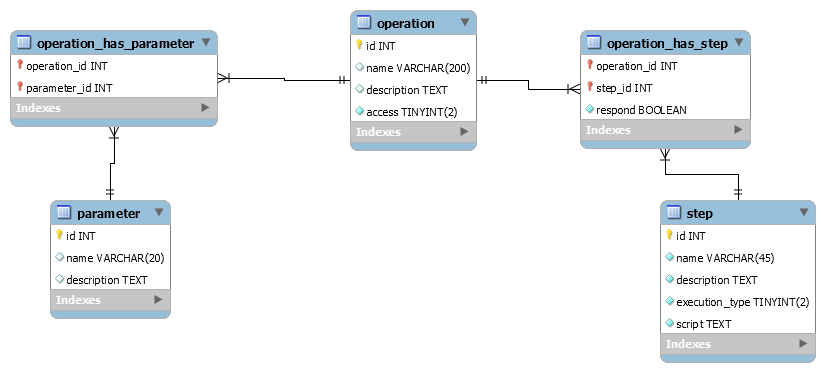
\includegraphics[width=1.0\textwidth]{DesarrolloInvestigacion/images/ModeloEntidadRelacion2.png}
    \caption{Modelo Entidad Relación del Motor}
\end{figure}
\begin{figure}[th!]
    \centering
    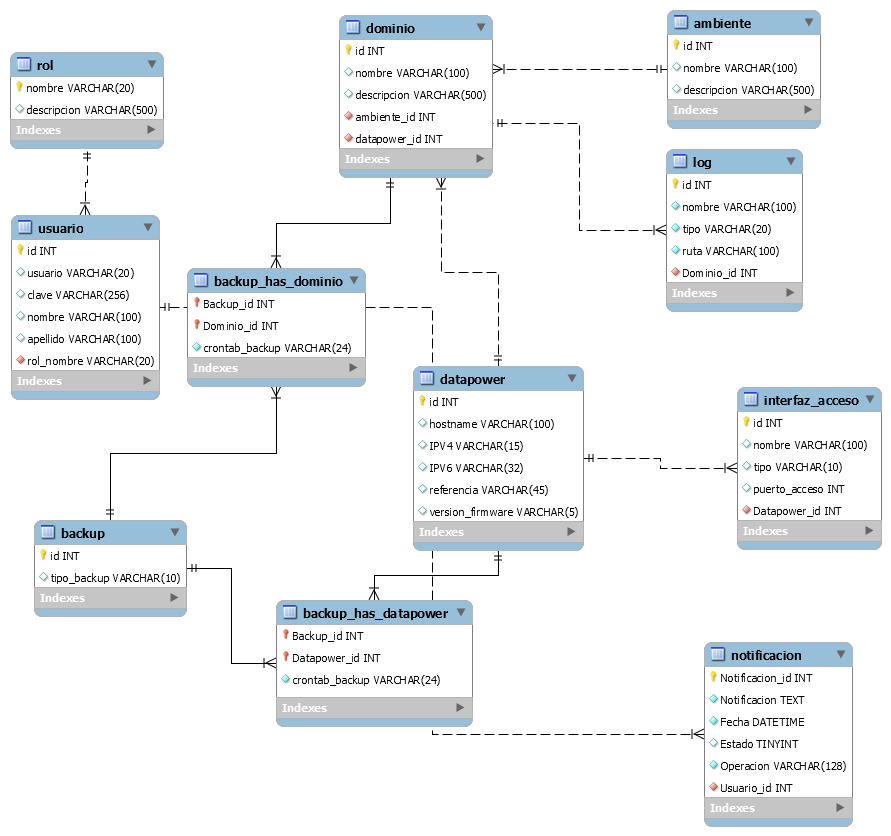
\includegraphics[width=1.0\textwidth]{DesarrolloInvestigacion/images/ModeloEntidadRelacion1.png}
    \caption{Modelo Entidad Relación de Administración}
\end{figure}

	\section{Descripcion Tecnica}
\subsection{Diagrama de despliegue}
\subsection{Herramientas y tecnologia}
	
	
	%\part{Arquitectura y Diseño}
%	\chapter{Descripción de la Organización}

\section{Introducción}
La empresa XAOP.DEV, desde su creación, ha pensado siempre en la calidad de los servicios que esta provee, tratando siempre de satisfacer más allá de lo que el cliente quiere.

\section{Descripción de la Organización}

\subsection{Misión}
Para el desarrollo de soluciones de tecnología de clase mundial, el logro de mejoras en el rendimiento del negocio de nuestros clientes, a través del uso de herramientas, procesos, metodologías y mejores prácticas que conducen a la implementación exitosa de proyectos de TI en calidad, tiempo y costo; sobre la base de un personal altamente competente.
\subsection{Visión}
Ser reconocidos en la industria como una compañía de alta tecnología, que ofrece soluciones y servicios de ingeniería a la medida, efectiva y con el apoyo de personal altamente cualificado, una tecnología constantemente actualizada, la innovación y la mejora continua de los procesos, para lograr un crecimiento sostenido que garantice su permanencia en el mercado.
%
%\subsection{Objetivos}
%\subsubsection{Misionales}
%\subsubsection{Estratégicos}
%\subsubsection{Operacionales}
%\section{Estructura Orgánica}
%\section{Funciones Organizacionales}
%\section{Procesos}
%\section{Servicios}
%\section{Productos}
	\section{Modelamiento arquitectura empresarial}
Archmate 2.0 facilita el modelado de la arquitectura empresarial, permitiendo bosquejar la organizacion desde diversos putnos de vista donde se reflejan tanto los involucrados en el negocio, la infraestructura y la misma solucion como los diferentes componentes, dando una vision general que describe a la perfeccion la organizacion y su solucion informatica.

XAOP.DEV una empresa en crecimiento de momento solo cuenta con el prototipo de administracion centralizada de Datapower, el cual se refleja en la presenta propuesta de arquitectura empresarial.

\newpage

\subsection{Punto de Vista Organizacional}
Este punto de vista se centra en la organización de una empresa, un departamento, una red de empresas o de una entidad. Es posible presentar los modelos en este putno de vista como diagramas de bloques anidades, sino tambien de una manera mas tradicional, tal como organigramas. El punto de vista organizacional es muy util en la identificacion de las competencias, la autoridad y las responsabilidades dentro de una organización.
\subsubsection{Modelo}
    \begin{figure}[th!]
        \centering
        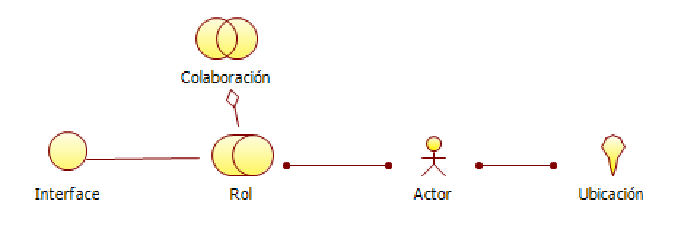
\includegraphics[width=1.0\textwidth]{Arquitectura/images/modelo/Punto_de_Vista_de_Organizacion.pdf}
        \caption{Modelo Punto de Vista Organizacional. . Fuente original}
    \end{figure}
\newpage
\subsubsection{Ejemplo}
    \begin{figure}[th!]
        \centering
        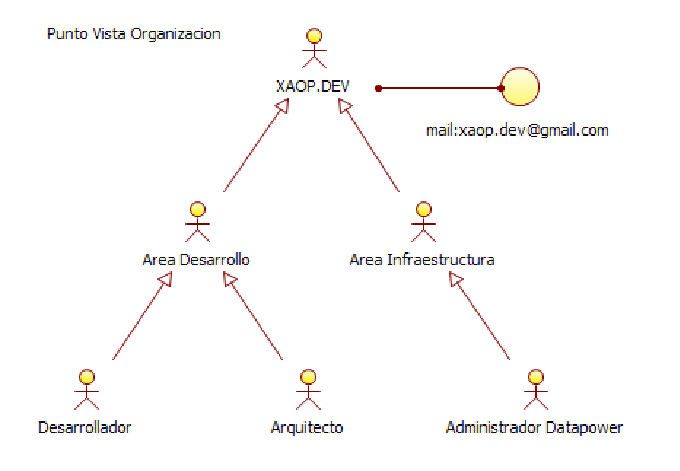
\includegraphics[width=1.0\textwidth]{Arquitectura/images/Punto_de_Vista_de_Organizacion.pdf}
        \caption{Ejemplo Punto de Vista Organizacional.}
    \end{figure}
\newpage

\subsection{Punto de Vista Cooperación de Actor}
Este punto de vista se centra en las relaciones de los actores entre si y su entorno. Un ejemplo comun es el diagrama de contexto, lo que pone una organizacion en su entorno, que consiste en las partes externas, tales como clientes, proveedores y otros socios comerciales. Es muy util en la determinacion de las dependientes externas y colaboraciones y mostrar la cadena de valor o de la red en el que opera el actor.
\subsubsection{Modelo}
    \begin{figure}[th!]
        \centering
        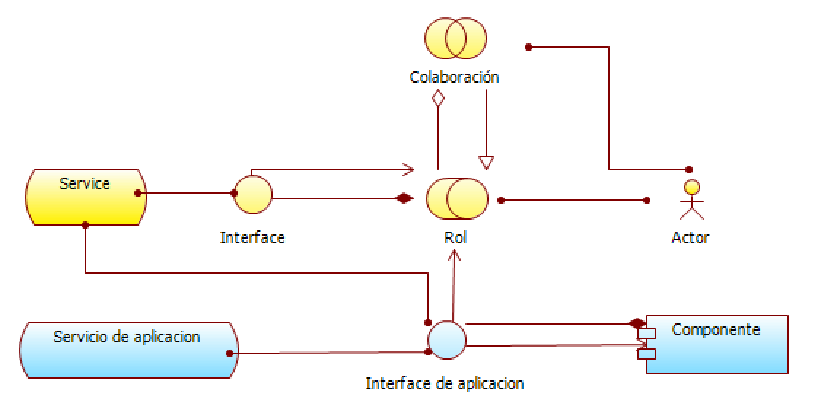
\includegraphics[width=1.0\textwidth]{Arquitectura/images/modelo/Punto_de_Vista_de_Cooperacion.pdf}
        \caption{Modelo Punto de Vista Cooperación de Actor}
    \end{figure}
\newpage
\subsubsection{Ejemplo}
    \begin{figure}[th!]
        \centering
        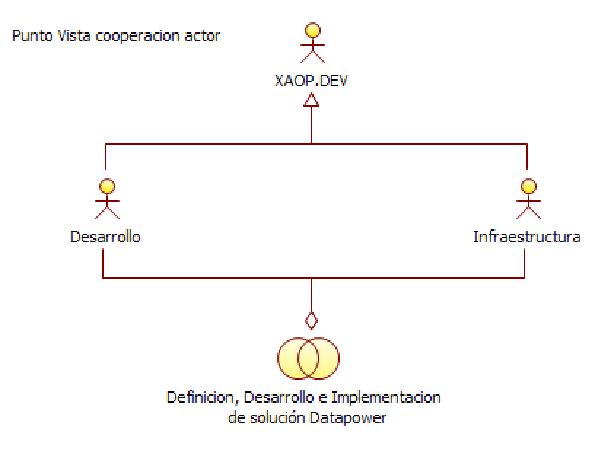
\includegraphics[width=1.0\textwidth]{Arquitectura/images/Punto_de_Vista_de_Cooperacion.pdf}
        \caption{Ejemplo Punto de Vista Cooperación de Actor}
    \end{figure}
\newpage

\subsection{Punto de Vista Función del Negocio}
Muestra las principales funciones de negocio de una organizacion y sus relaciones en terminos de los flujos de informacion, el valor, y cosas entre ellos. Las funciones de la empresa seutilizan para representar los aspectos mas estables de una empresa en terminos de las actividades primarias que realiza, independientemente de los cambios de organizacion o desarrolos tecnologicos.
\subsubsection{Modelo}
    \begin{figure}[th!]
        \centering
        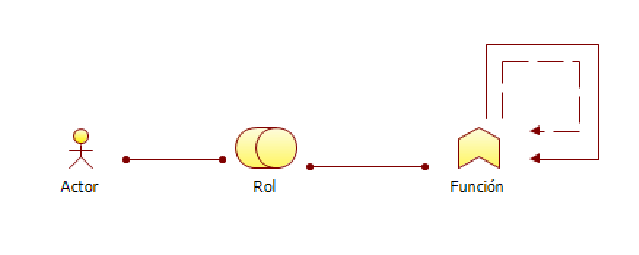
\includegraphics[width=1.0\textwidth]{Arquitectura/images/modelo/Punto_de_Vista_de_Funcion_del_Negocio.pdf}
        \caption{Modelo Punto de Vista Funcion del Negocio}
    \end{figure}
\newpage
\subsubsection{Ejemplo}
    \begin{figure}[th!]
        \centering
        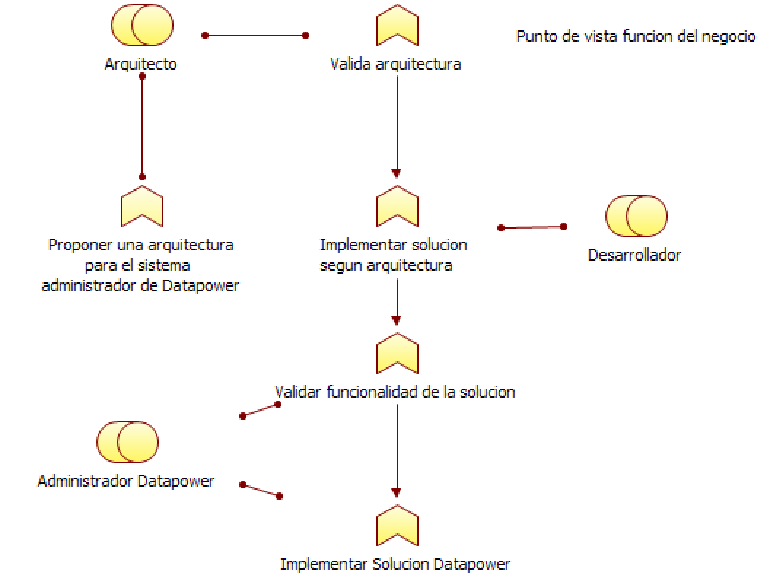
\includegraphics[width=1.0\textwidth]{Arquitectura/images/Punto_de_Vista_de_Funcion_del_Negocio.pdf}
        \caption{Ejemplo Punto de Vista Funcion del Negocio}
    \end{figure}
\newpage

\subsection{Punto de Vista Proceso del Negocio}
Se utiliza para mostrar la estructura de alto nuvel y la composicion de un o mas procesos de negocio.
\subsubsection{Modelo}
    \begin{figure}[th!]
        \centering
        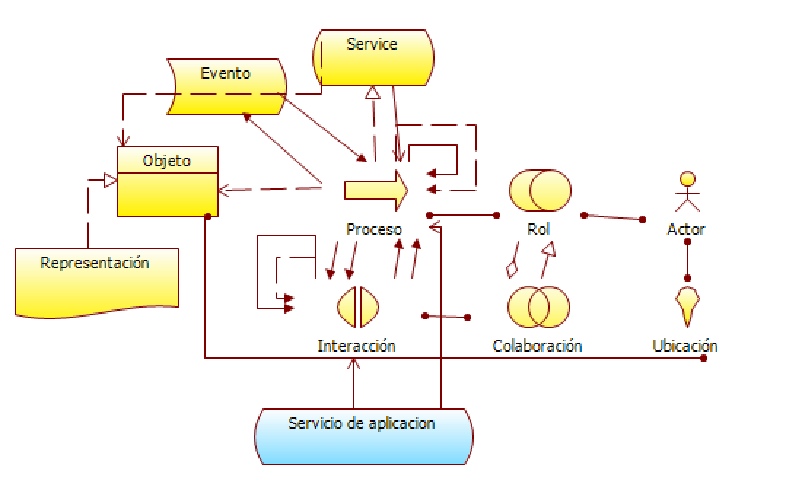
\includegraphics[width=1.0\textwidth]{Arquitectura/images/modelo/Punto_de_Vista_de_Proceso_de_Negocio.pdf}
        \caption{Modelo Punto de Vista Proceso del Negocio}
    \end{figure}
\newpage
\subsubsection{Ejemplo}
    \begin{figure}[th!]
        \centering
        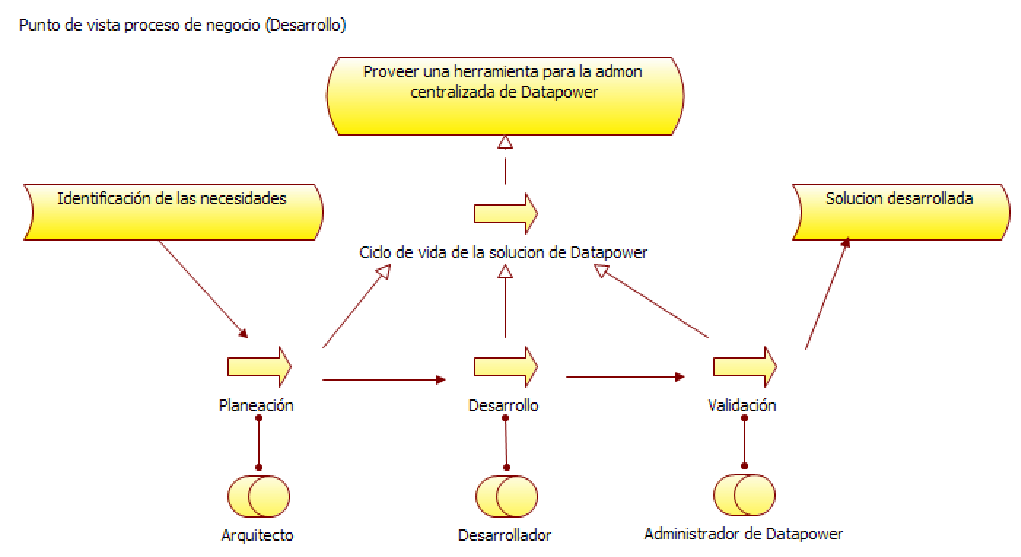
\includegraphics[width=1.0\textwidth]{Arquitectura/images/Punto_de_Vista_de_Proceso_de_Negocio_Desarrollo.pdf}
        \caption{Ejemplo Punto de Vista Proceso del Negocio (Desarrollo)}
    \end{figure}
\newpage
\subsubsection{Ejemplo}
    \begin{figure}[th!]
        \centering
        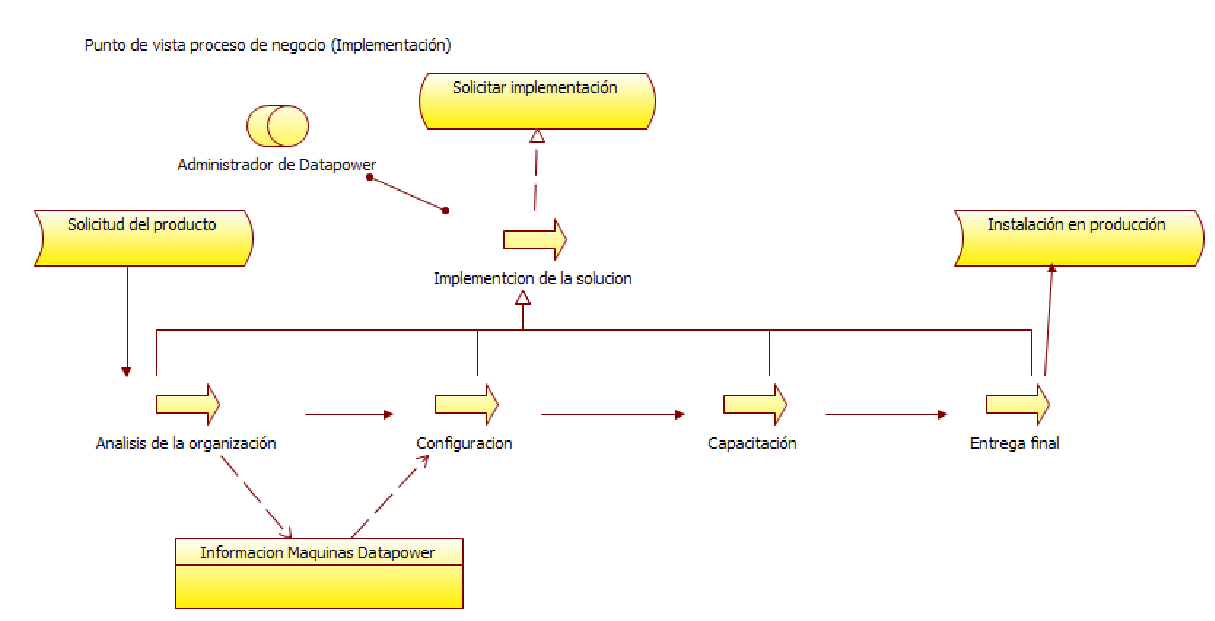
\includegraphics[width=1.0\textwidth]{Arquitectura/images/Punto_de_Vista_de_Proceso_de_Negocio_Implementacion.pdf}
        \caption{Ejemplo Punto de Vista Proceso del Negocio (Implementacion)}
    \end{figure}
\newpage

\subsection{Punto de Vista Producto}
El punto de vista del producto representa el valor que el producto ofrece para los clientes y muestra como esta compuesto el producto que se esta ofreciendo, representa cada uno de los modulos por los que se compone la solución.
\subsubsection{Modelo}
    \begin{figure}[th!]
        \centering
        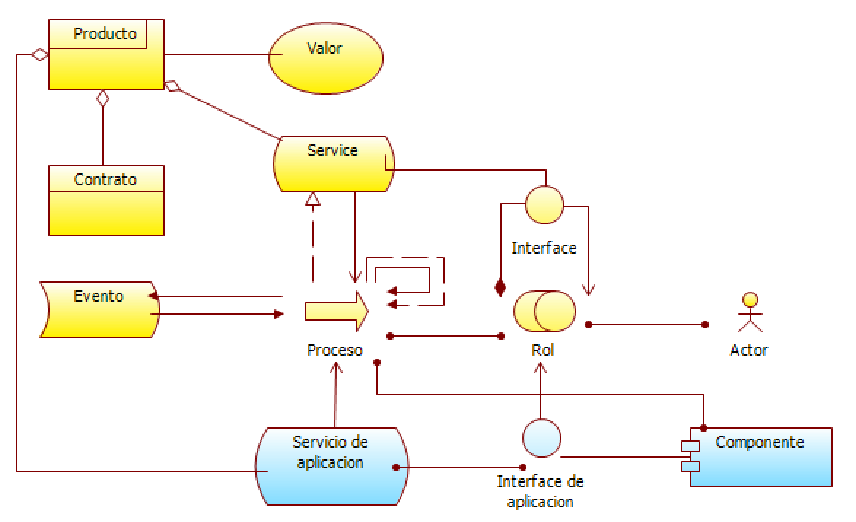
\includegraphics[width=1.0\textwidth]{Arquitectura/images/modelo/Punto_de_vista_Producto.pdf}
        \caption{Modelo Punto de Vista Producto}
    \end{figure}
\newpage
\subsubsection{Ejemplo}
    \begin{figure}[th!]
        \centering
        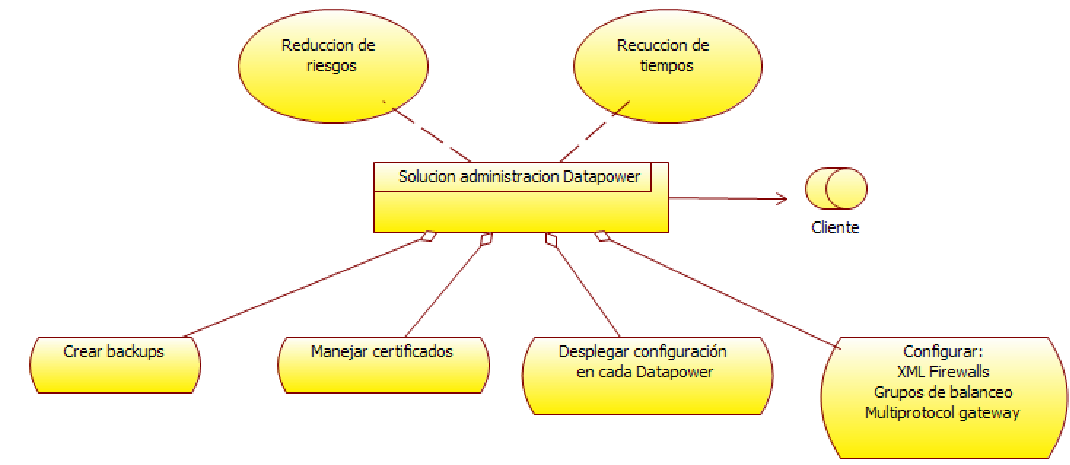
\includegraphics[width=1.0\textwidth]{Arquitectura/images/Punto_de_vista_Producto.pdf}
        \caption{Ejemplo Punto de Vista Producto}
    \end{figure}
\newpage
	\include{Arquitectura/cap5}
	
	%\part{Conclusiones y Anexos}
	\chapter{Cierre de la investigación}
\section{Resultados y discusión}
\section{Conclusiones}
%%%%%%%%%%%%%
%%carretazo aqui
%%%%%%%%%%%%%
\subsection{Verificación, contraste y evaluación de los objetivos}
\begin{itemize}
    \item La administración de la infraestructura en una organización es algo crucial para el negocio, por esto mismo es importante que los administradores cuenten con herramientas y facilidades para realizar su labor del día a día de un modo mas sencillo y certero.
    \item El conjunto de operaciones administrativas que realiza cada administrador de maquinas Datapower es diverso, ya que este, se encuentra atado a la implementación que se haya realizado en su organización, por ello es necesario brindar una herramienta con un alto grado de parametrización.
\end{itemize}
\subsection{Síntesis del modelo propuesto}
\subsection{Aportes originales}

	\chapter{Prospectiva del trabajo de grado}
\newpage
\section{Prospectiva del trabajo de grado}
%%%%%%%%%%
%%carreta aqui
%%%%%%%%%%
\subsection{Trabajos de investigación futuros}
\begin{itemize}
    \item La proyección que se tiene para futuros desarrollos es poder presentar una herramienta altamente parametrizable, de forma que cada organización parametrize sus tareas y usen la herramienta con tareas que usan habitualmente, con posibilidad de ampliar la funcionalidad.
    \item Otra de las características fundamentales para cualquier organización es el manejo de estadísticas que le ayuden a observar el comportamiento de las maquinas administradas por la solución. Es por eso que otra de las funcionalidades adicionales es el reporte de estadísticas que genere cada tarea independiente.
\end{itemize}
	\chapter*{Anexos}

\definecolor{dkgreen}{rgb}{0,0.6,0}
\definecolor{gray}{rgb}{0.5,0.5,0.5}
\definecolor{mauve}{rgb}{0.58,0,0.82}

\lstset{frame=tb,
	language=Java,
	aboveskip=3mm,
	belowskip=3mm,
	showstringspaces=false,
	columns=flexible,
	basicstyle={\small\ttfamily},
	numbers=none,
	numberstyle=\tiny\color{gray},
	keywordstyle=\color{blue},
	commentstyle=\color{dkgreen},
	stringstyle=\color{mauve},
	breaklines=true,
	breakatwhitespace=true,
	tabsize=3
}
	
	%bibliografia
    \bibliographystyle{apalike}
    \bibliography{articulos,libros}
\end{document}